\documentclass{article}

\title{P6 Report}
\author{Nick Werle}

\usepackage{hyperref}
\usepackage{graphicx}

\begin{document}
\maketitle
\section{Preamble}
All necessary files will be uploaded to my githb repository at \url{https://github.com/NickWer/CEG3900_P6}

\section{Task 1}
I created four ubuntu server instances on AWS EC2 and then manually segmented each file into 13 rows (52 hashes to begin).
I let the four instances of John run for ~3 hours and managed, as expected to crack the guest password (guest007).

At this time I haven't started the android APK - it's unclear how I'm going to make it run.
That is, I think it won't be bad to start the process, but I'm unsure how I will be able to get the output/list collected passwords.
Perhaps two buttons - one that starts john, the other that runs `john --show etc-shadow-2009.txt` and returns that output.

	\begin{figure}[ht]
        \centerline{
            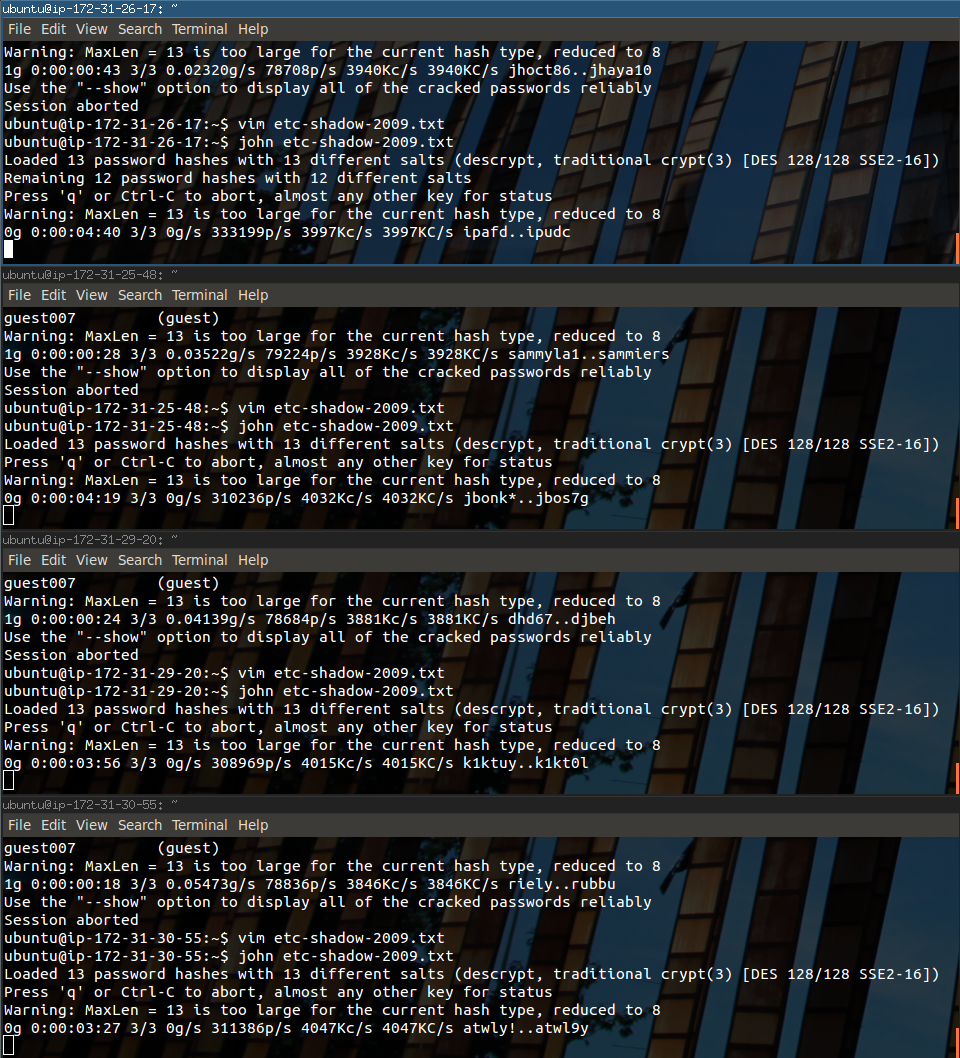
\includegraphics[width=7.5in]{img/t1s1.png}
        }
		\centering
		\caption{Task 1 - Four instances running at once over ssh}
	\end{figure}


\clearpage

\section{Task 2}
I was able to run hashcat on my desktop at home, which natively runs Ubuntu 16.04 (as opposed to my laptop that I `dist-uprade`ed to 16.04), and also includes an NVidia GPU as opposed to my laptop's AMD card.

\end{document}
